\documentclass{article}
\usepackage[utf8]{inputenc}
\usepackage{biblatex}
\addbibresource{bibliography.bib}
\usepackage{graphicx}
\usepackage{subcaption}
\usepackage{caption}
\usepackage{siunitx}
\usepackage{hyperref}
\graphicspath{{./images/}}

\usepackage[a4paper, total={6.5in, 8in}]{geometry}
\usepackage[left]{lineno}
\linenumbers

\bibliography{bibliography}

\newcommand*{\ts}{{\tau^{*}}}
\newcommand*{\diff}{\mathop{}\!\mathrm{d}}
\newcommand{\ps}{\si{\pico\second}}
\newcommand{\ns}{\si{\nano\second}}
\newcommand{\fs}{\si{\femto\second}}
\newcommand{\ips}{\si{\per\pico\second}}
\newcommand{\us}{\si{\micro\second}} 
\newcommand{\iA}{\si{\per\angstrom}}
\newcommand{\K}{\si{\kelvin}} 

\title{The application of the generalised Langevin equation to surface diffusion and the effect of noise correlations on low-friction activated diffusion processes.}

\author{Jeremy Wilkinson}
\date{September 2021}

\begin{document}

\maketitle

\begin{abstract}
    mucho cool langevin
\end{abstract}

\tableofcontents

\section{Introduction}

Understanding the motion of adsorbed particles over the surface of a substrate is of interest to many fields. Experimental techniques such as helium spin echo microscopy provide insight into adsorbate motion of real systems over a wide range of time and length scales. Current experimentally observable quantities, such as the intermediate scattering function, do not provide direct measurements of individual adsorbate trajectories. It is therefore common practice to introduce models for the microscopic motion of adsorbates to assist in the data interpretation process. 

Molecular dynamics simulations modelling the substrate lattice, adsorbate and their interactions have been used to fit experimental data. This approach has the advantage of capturing the classical phonon-adsorbate interaction entirely. One particular drawback of this approach is the large computational cost associated with simulating the pairwise interactions of thousands of substrate atoms and the adsorbate. 

Langevin dynamics provide an alternative, computationally efficient, approach to modelling inherently chaotic simulations by treating the forces seen by the adsorbate as stochastic and ommiting the substrate from the simulation entirely. Previous work has used the Markovian Langevin equation to succesfully fit the observables of both molecular dynamics and experimental data. However certain anomolous effects such as the temperature dependent friction reported by M Diamant et al suggest there may be discrepencies between molecular dynamics simulations and the Markovian Langevin equation. This paper investigates the effect of removing the Markovian constraint on the stochastic force in the Langevin equation through the use of the generalised Langevin equation and to quantify the effects this has on activated diffusion in the low friction regime. 

\section{Langevin dynamics} \label{sec:langevin}

The Markovian Langevin equation describes the time evolution of a degree of freedom, such as a particle's position, in the presence of a large chaotic system. The Langevin equation formalises the notion that the influence of a sufficiently chaotic system on surrounding particles is, for all intents and purposes, a random variable with equilibrium statistical properties set by the ergodic hypothesis\footnote{A formal development of the Langevin hypothesis may be found in \cite{Kramers}.}. A particle is said to obey Markovian Langevin statistics if the force it experiences obeys the stochastic differential equation,
\\
\begin{equation}
	\label{eq:markovian_le}
	m\ddot{x}(t)=-m\eta\dot{x}(t) - \nabla U(x(t)) + f(t) \text{ and } \left<f(t_1)f(t_2)\right>=2k_BTm\eta\delta(t_1 - t_2)
\end{equation}
\\
for some friction constant $\eta$. The second equality in Equation \ref{eq:markovian_le}, known as the fluctuation-dissipation theorem, ensures that the particle obeys the equipartition theorem and states that the noise in the system is uncorrelated in time. In the frequency domain, this condition is equivelant to a uniform power spectral density, $\left<\tilde{f}(\omega_1)\tilde{f}(\omega_2)\right>=2k_BTm\eta2\pi\delta(\omega_1 + \omega_2)$ and is consequently reffered to as white noise. The statistical physics of Equation \ref{eq:markovian_le} is well understood and can be shown to satisfy equilibrium boltzmann statistics, $\rho(x, p)=\frac{1}{Z}\exp(-\beta H(x, p))=\frac{1}{Z}\exp(-\beta(p^2/2m + U(x)))$, exactly for an arbitrary background potential $U(x)$ provided $f$ is a gaussian random variable.

While the Markovian Langevin equation is useful due to its analytic simplicity, the noise in all physical systems is bandlimited and therefore a particle experiences noise correlations in time. One may introduce a memory kernel, $K(t)$, into the Langevin equation to capture these correlations but this modification requires a corresponding change to the friction term to ensure equipartition of energy. This results in the non-Markovian Langevin equation, $m\ddot{x}(t)=-m\eta\int\diff{t'}\dot{x}(t')K(t-t') + \int\diff{t'}f(t')K(t-t')$, which obeys boltzmann statistics exactly in a flat background potential for any memory kernel normalised to have a total area of $1$ (the statistics of $f$ remain unchanged). However once a background potential is added to the non-Markovian Langevin equation,
\\
\begin{equation}
	\label{eq:gle}
	m\ddot{x}(t)=-m\eta\int\diff{t'}\dot{x}(t')K(t-t') - \nabla U(x) + \int\diff{t'}f(t')K(t-t'),
\end{equation}
\\
analytical results become sparse and the assumption that the fluctuation dissipation condition is sufficient to ensure equipartition of energy becomes an approximation. Fortunately it is often a reasonable approximation to make although it is not difficult to construct situations that demonstrate its failure. 

While the form of $K(t)$ is left unconstrained, an exponential memory kernel of the form $K(t)=\theta(t)\frac{1}{\tau}\exp\left(-\frac{t}{\tau}\right)$\footnote{$\theta(t)$ is used here to denote the Heaviside step function.}, parametrized by the correlation time $\tau$, has the advantage of being extremely computationally efficient as one can perform convolutions in linear time through the relation
\\
$$
\int_0^{n\Delta{t}} dt' K\left(t-t'\right) \vec{f}(t') \approx \alpha \int_0^{(n-1)\Delta{t}} dt' K\left(t-t'\right) \vec{f}(t') + \frac{1}{1-\alpha} \vec{f}\left(t_n\right)
$$
\\
where the decay factor $\alpha$ is given by $\alpha=\exp(-\frac{\Delta{t}}{\tau})$ for a simulation of timestep $\Delta{t}$. The power spectrum of $K(t)$ is given by $\left|\tilde{K}(\omega)\right|^2 = \frac{1}{1+\omega^2\tau^2}$ with bandwidth given by the half-width at half-maximum, $w_c=\frac{1}{\tau}$.

\begin{figure}
	\centering
	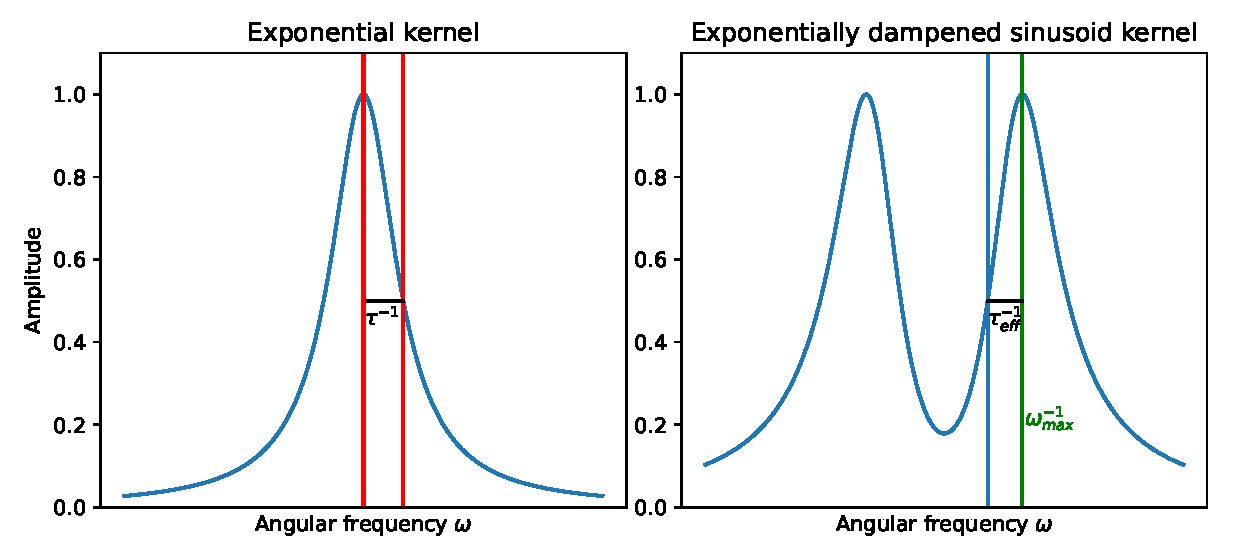
\includegraphics[width=0.5\textwidth]{kernel_spectra}
	\caption{The power spectrum of the exponential kernel is centered around $0$ with a half-width at half-maximum of $\tau^{-1}$.}
	\label{fig:kernel_spectra}
\end{figure}

\section{Experimentally observable quantities and methods for interpretation}

The motion of an absorbate over a surface may be quantified through the use of the van Howe pair correlation function. For a single adatom present on a surface, the van Howe pair correlation function coincides with the probability, $P\left(\vec{r},t\right)$, of finding the adatom at position $\vec{r}$ at time $t$ given that it was present at the origin at $t=0$. The directly observeable quantity in a scattering experiment is the spatial Fourier transform of the van Howe pair correlation function known as the intermediate scattering function (ISF) given by $ISF\left(\Delta{\vec{K}}, t\right) = \int \diff{\vec{r}} \exp\left(-i\Delta{\vec{K}}\cdot\vec{r}\right)P(\vec{r}, t)$. This quantity also happens to be simple to extract from simulated trajectories and forms the basis of the analysis in this paper. Within the context of a surface scattering experiment, the argument $\Delta{\vec{K}}$ is referred to as `the momentum transfer' as this quantity corresponds to the momentum transferred to the surface in the process of scattering. The ISF is often only quoted in terms of the 2D component of the momentum transfer parallel to the surface as most devices which measure physical ISFs are insensitive to the fast scale motion in the direction perpendicular to the surface.

Figure \ref{fig:isf_example} shows a typical ISF for a fixed momentum transfer as a function of time. The typical features include a sharp drop with oscillations at short times that correspond to intracell motion of the adsorbate as it explores its local adsorbtion site. At longer times, the ISF typically exhibits an exponentially decaying tail with decay rate denoted by $\Gamma$. For most isolated adatoms on a bravais lattice, this tail is given by the mean square distance in the direction of $\Delta{\vec{K}}$, $ISF(t) \sim \exp\left(- \left<\left(\Delta{\vec{K}}\cdot\vec{r}(t)\right)^2\right>\right)$. The mean square distance of an adatom performing random hops is asymptotically linear and proportional to the hopping rate, $\gamma$. $\Gamma$ is therefore proportional to the hopping rate of the adatom, a familiar fact from the Chudley-Elliot model of jump diffusion.

\begin{figure}
	\centering
	\includegraphics[width=0.5\textwidth]{isf_example}
	\caption{}
	\label{fig:isf_example}
\end{figure}

\subsection{Understanding the factors influencing the hopping rate $\gamma$}

Consider a particle weakly coupled to a heat bath trapped by a potential barrier of height $E_a$. The rate of escape of the particle is a sophisticated quantity which is difficult to understand from first principals. Each time the particle finds itself with enough energy to escape the barrier, one imagines it has a certain probability of finding the bridge point before interactions with the heat bath cause a shift to a new independent energy level, likely less than the barrier energy. This line of reasoning justifies the factorization of the hopping rate into the product of the rate at which the particle explores energy levels, the probability that a given energy level is greater than $E_a$, and the probability that the particle will find a bridge point before its energy changes. The number of independent energy levels attained per unit time is quantified through the reciprocal of the typical correlation time of the total energy of the particle, reffered to as the \emph{time to forget}, $\phi$. On the other hand, the probability of attaining an energy level greater than $E_a$ is dictated by Boltzmann statistics whereas the probability of escape is a complex quantity which for the purposes of this paper will simply be treated as a functional of the potential energy background. The validity of this factorization should not be taken too seriously without further justification but is helpful in understanding the effects involved in low friction activated diffusion. 

First principal calculations for the escape rate of a Markovian Langevin particle from a trapping well have been studied for many decades. A particle in an approximately harmonic trap of natural frequency $\omega_0$ and barrier height $E_a$, in the low friction regime ($\frac{\eta}{\omega_0} << 1$), has an Ahrrenius form,
\begin{equation}
	\gamma = A \eta \exp\left(-\beta E_a \right)
	\label{eq:ahrrenius}
\end{equation}
which is observed in both experimental data and simulated models. The total energy autocorrelation function of a Markovian Langevin particle in a 1D harmonic well is given by $\left<E(0)E(t)\right> = (1 + \exp(-\eta t)) (k_BT)^2$ and therefore has a time to forget of $\eta^{-1}$. Equation \ref{eq:ahrrenius} therefore manifests the aforementioned factorization, with the energy exploration rate $\phi^{-1}=\eta$, the probability of attaining sufficient energy proportional to $\exp(-\beta E_a)$ and $A$ containing the probability of escape as well as any other constants.

\section{Computational evaluation of activated diffusion in the presence of noise correlations}

A 2D non-Markovian Langevin simulation with an exponential memory kernel was constructed, as described in Section \ref{sec:langevin}. The background potential, Figure \ref{fig:pot_surface}, was extracted from the free energy of a molecular dynamics simulation of Sodium on Copper(001) as described in \cite{Gil}. The simulation was found to obey the expected Ahrrenius law with an activation energy of $something$ consistent with ?? as well as an ISF decay rate, $\Gamma$, proportional to $\eta$, consistent with the theoretical developments thus far.

The simulation was run for each combination of $\eta \in \left(0.4, 0.41 \dots 0.79\right)$ and $\tau \in \left(0.0, 0.01 \dots 0.39\right)$ for $2\us$ at $300\K$ with a timestep of $1\fs$. The position and total energy of the adatom was recorded at each timestep and used to construct the ISF and total energy autocorrelation function for each simulation.

\begin{figure}
	\centering
	\begin{subfigure}{0.59\textwidth}
		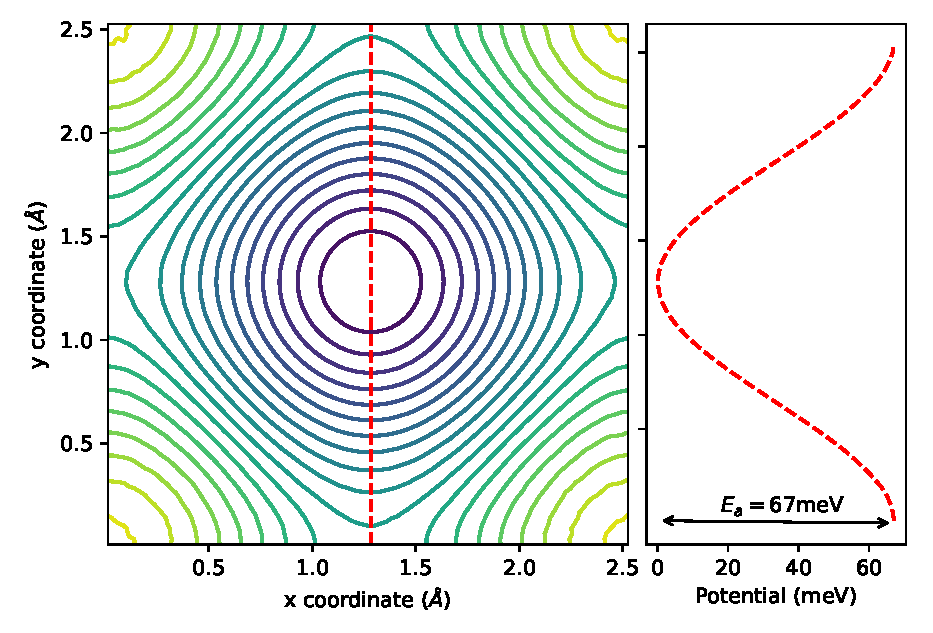
\includegraphics[width=1.0\textwidth]{pot_surface}
		\caption{The unit cell potential background used to tile the plane for the 2D Langevin simulations. The potential has a local harmonic approximation of natural frequency $\omega_0=8.8\ips$}
		\label{fig:pot_surface}
	\end{subfigure}
	\begin{subfigure}{0.39\textwidth}
		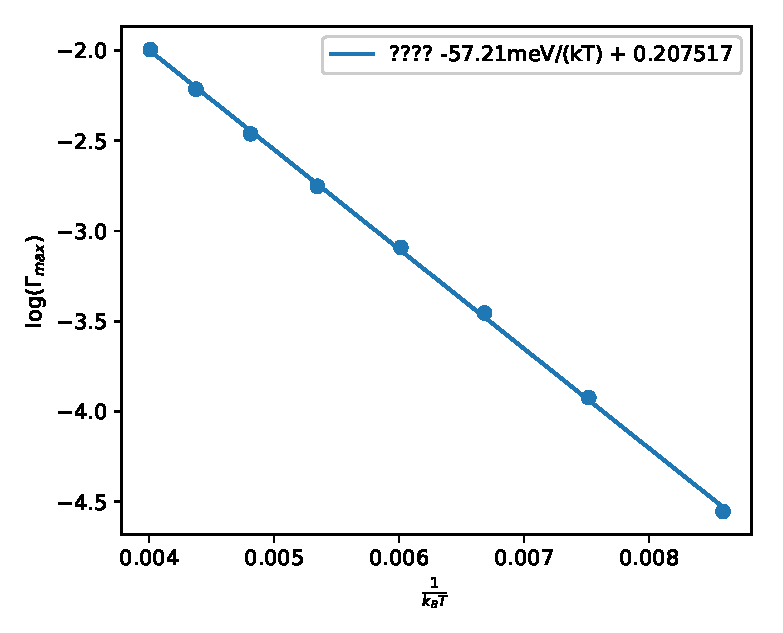
\includegraphics[width=1.0\textwidth]{ahrrenius}
		\caption{}
		\label{fig:ahrrenius}
	\end{subfigure}
\end{figure}

\subsection{The effect of noise correlations on $\Gamma$}

The long-time ISF decay rate, $\Gamma$, was extracted from the ISF in the $(110)$ crystal azimuth for each simulation and the results of this process are summarized in Figure \ref{fig:eta_tau_gamma}. As expected, for low $\tau$ the ISF dephasing rate is linear in the friction constant. However it is observed that this trend continues as $\tau$ becomes significant albeit with a decreasing gradient. Secondly it is clear that noise correlations can have a significant effect on the ISF dephasing rate with $\Gamma$ decreasing by a factor of four as $\tau$ varies between $0$ and $0.4\ps$.

If one considers increasing $\tau$ from $0$, extremely high frequency components in the noise power spectrum are the first to be suppresed. The panel on the right of Figure \ref{fig:eta_tau_gamma} demonstrates that the effect of these high frequency components on $\Gamma$ are negligable as they are higher order in $\tau$. This is perhaps not surprising as extremely high frequency noise components average out quickly on the timescale of adatom motion over the potential background and leave the macroscopic trajectory unchanged. The averaging out of high frequency noise components has been observed before in the context of diffusion without a background potential \cite{Townsend}, however in this case the result is trivial as the Fourier spectrum of the particle's trajectory, $\vec{x}(t)$, is linear in the noise power spectrum. 

The existance of a maximum relevant frequency threshold for long time-scale observables in the simulation is an important feature as no simulation can contain frequency components greater than $\frac{1}{2\Delta{t}}$. So if these noise components were important, then no digitial simulation could faithfully reproduce even the long-time observables of a Langevin equation. The flip side of this is also a consideration since decreasing the timestep in a Markovian Langevin simulation might otherwise noise components with observable effects. Therefore systems in which the noise cutoff is close to or below the maximum relevant frequency require a careful determination of the simulation timestep, or the use of the non-Markovian Langevin equation in order to behave as intended.

\begin{figure}
	\centering
	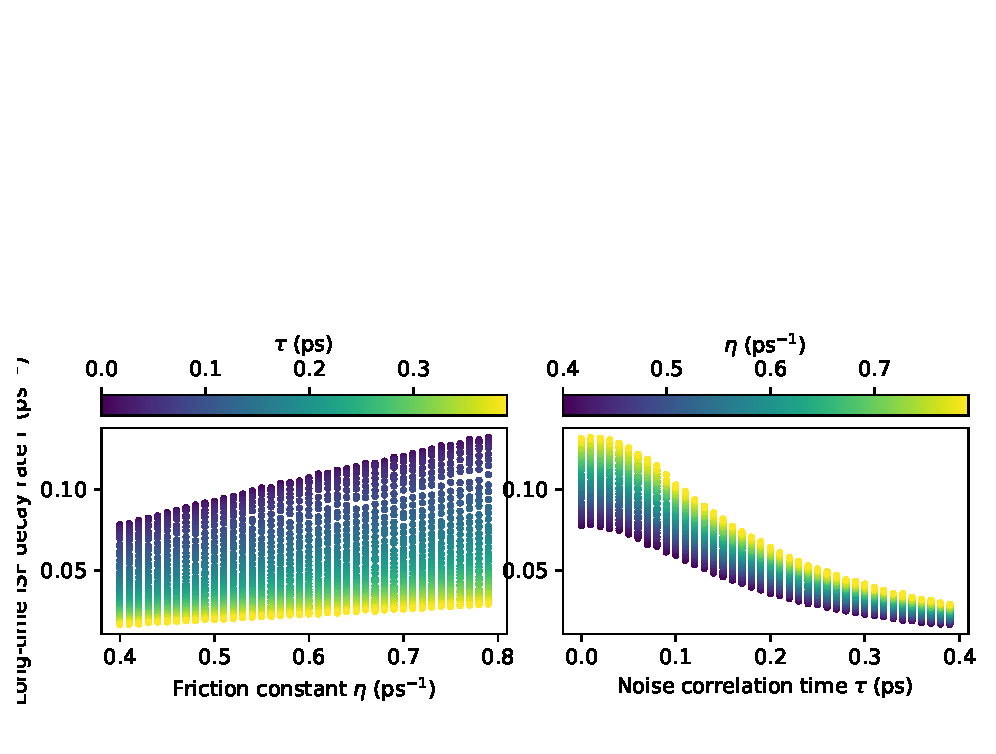
\includegraphics[width=1.0\textwidth]{eta_tau_gamma}
	\caption{Scatter plots of the dephasing rate of simulated ISFs in the $(110)$ crystal azimuth with a momentum transfer of $\left|\Delta{K}\right|=1.23\iA$.} 
	\label{fig:eta_tau_gamma}
\end{figure}

\subsection{The effect of noise correlations on $\phi$}\label{sec:phi}

Figure \ref{fig:eta_tau_ttf} shows the decay rate of the total energy autocorrelation function, $\phi^{-1}$, extracted from each simulation as a function of $\eta$ and $\tau$. The total energy dephasing rate is seen to have a similar, strong dependence on $\tau$ as in the case of $\Gamma$. The striking similarity of the trends in Figure \ref{fig:eta_tau_ttf} to those in \ref{fig:eta_tau_gamma} are indicative of the fact that the $\Gamma$ is in fact a function of the time to forget, $\phi$, and not of $\eta$ directly. Figure \ref{fig:gamma_and_ttf_scatter} demonstrates this point further and shows the almost linear relationship between $\Gamma$ and $\phi^{-1}$. The deviation from perfect linearity is likely due small dependences of the other factors in $\Gamma$ on $\phi$, for example one would expect the probability of escape given enough energy to be somewhat dependent on the amount of time spent at that energy level. 

\begin{figure}
	\centering
	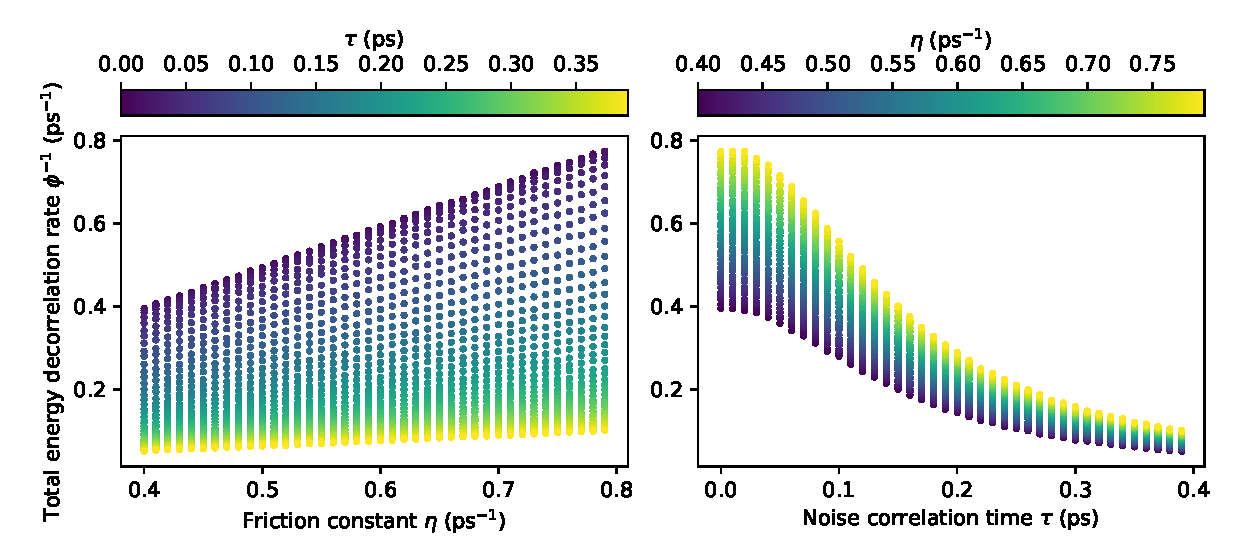
\includegraphics[width=1.0\textwidth]{eta_tau_ttf}
	\caption{Scatter plots of the total energy dephasing rate of the adatom vs $\eta$ \& $\tau$. } 
	\label{fig:eta_tau_ttf}
\end{figure}


\begin{figure}
	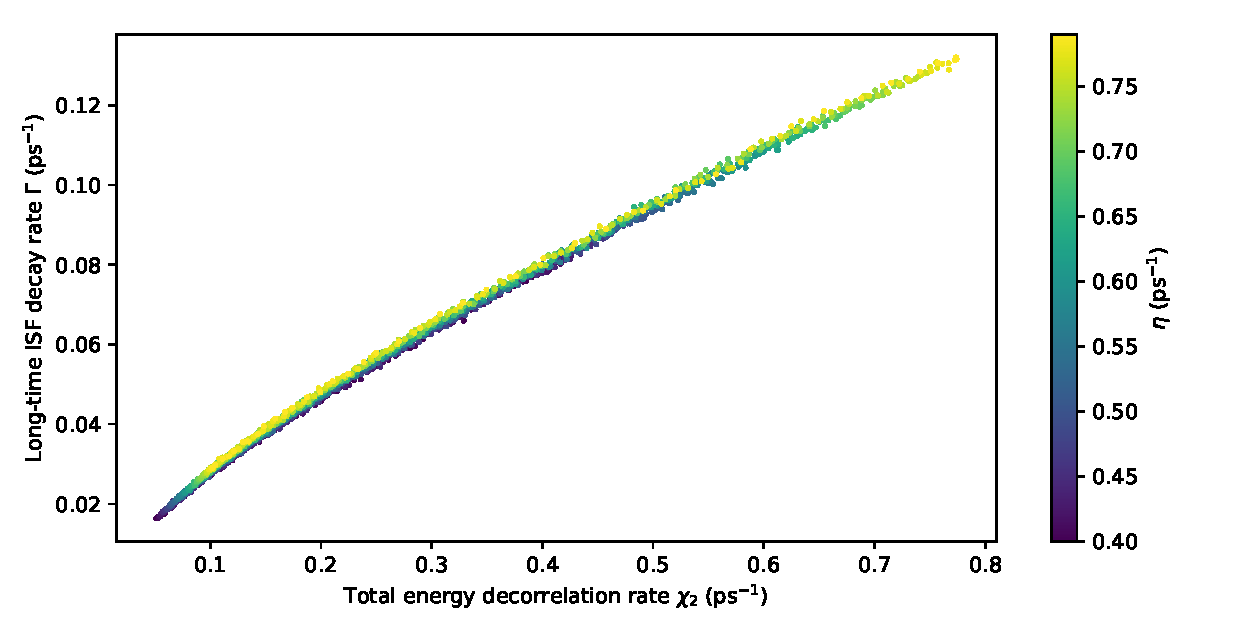
\includegraphics[width=1.0\textwidth]{gamma_and_ttf_scatter}
	\caption{The relationship between the total energy decay rate $\phi^{-1}$ and the ISF decay rate $\Gamma$ is observed to be linear except in the small $\phi^{-1}$ limit. The colour of each marker is set by the value of $\eta$ for the simulation and further demonstrates that $\Gamma$ is not solely function of $\eta$.}
	\label{fig:gamma_and_ttf_scatter}
\end{figure}


\subsection{The effect on the jump distribution}

Since Figure \ref{fig:gamma_and_ttf_scatter} showed that, in the $\eta$-$\tau$ plane, $\Gamma$ is solely a function of $\phi$, one might wonder whether the orthogonal parameter has an effect on any observables. Another observable used to fit experimental data is the so-called jump distribution. To check whether the orthogonal parameter has an effect on the jump distribution, a $2\us$, $300\K$ simulation was run for a series of parameters which held $\phi$ fixed but allowed $\eta$ and $\tau$ to vary. Due to small errors in the determination of the the values of $\eta$ and $\tau$ required to hold $\phi$ fixed, the normalization of the jump distributions was fixed to peak at $1.0$ to aid in comparing the shapes of the jump distributions. Figure \ref{fig:jump_distributions} shows the resulting normalized jump distributions with the un-normalized curves inset for completeness. The shape and therefore spectral content of the jump distributions are observed to agree within experimental accuracy. Therefore it appears that the time to forget is also the determining factor for the relative probability of single vs multijumps in the simulation. This is in contrast to the sharper peaks observed in the jump distributions in \cite{Gil} for larger $\eta$, indicating that higher friction was responsible for prodimenantly single jumps.

\begin{figure}
	\centering
	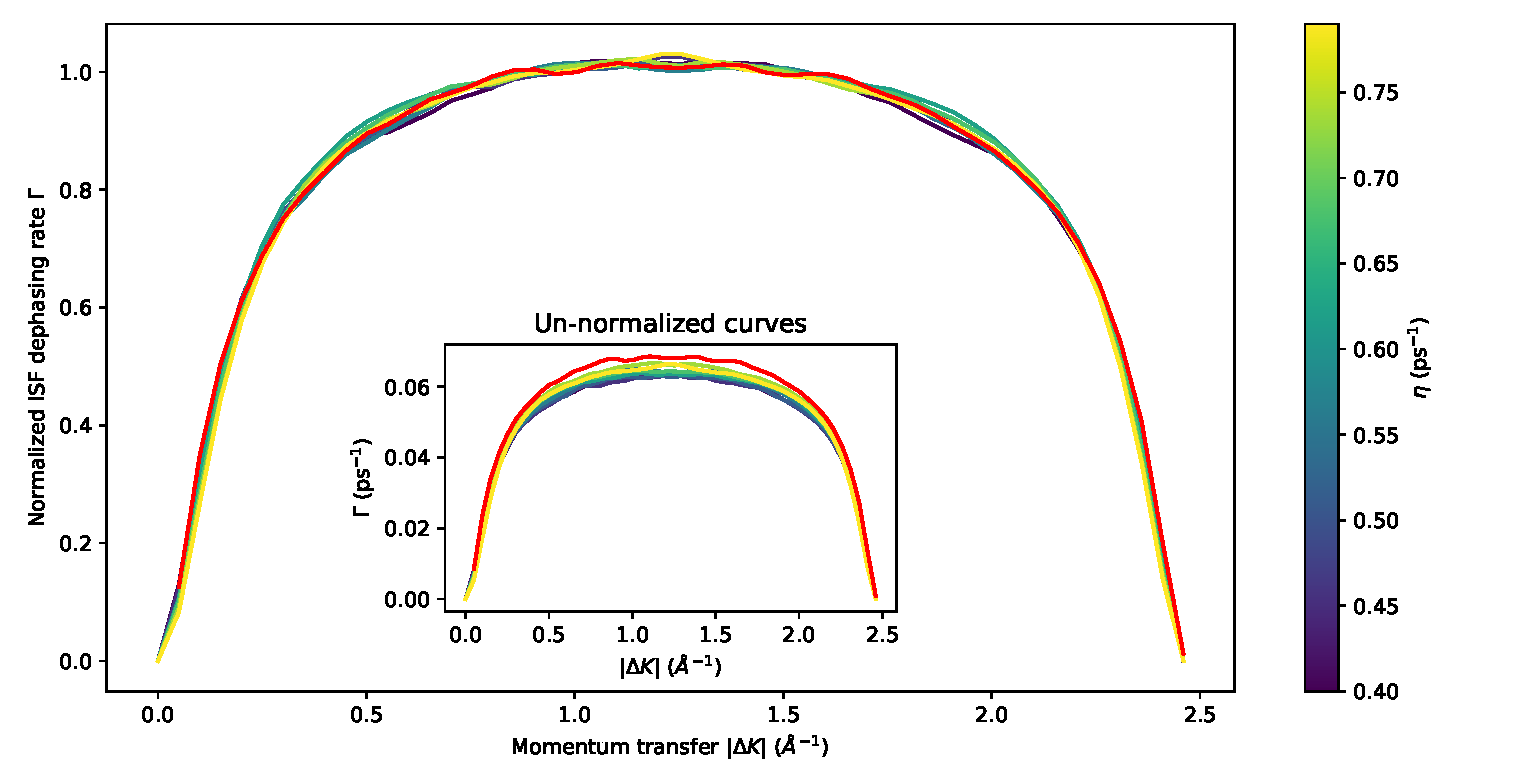
\includegraphics[width=1.0\textwidth]{jump_distributions}
	\caption{Results of a series of simulations in which $\phi^{-1}$ was held fixed at approximately $0.285\ips$ using the values of $(\tau,\eta)\in\left\{(0.4, 0.0862), (0.45, 0.1065), (0.5, 0.1236), (0.55, 0.1384), (0.6, 0.1514), (0.65, 0.164), (0.7, 0.1759), (0.75, 0.1867)\right\}$ . The inset figure shows the jump distributions for these simulations and the main figure shows the same curves normalized to peak at $1.0$ to aid in the comparison of the jump distribution shapes.}
	\label{fig:jump_distributions}
\end{figure}

\subsection{Theoretical results for the time to forget in a harmonic well}

The results so far demonstrate the time to forget of the system appears to be an important parameter in the determination of various high-level observables. $\phi^{-1}$ has also been observed to be linear in $\eta$ over the investigated parameter range. In principal, $\phi$ may be a complicated functional of the background potential, and the other constants in the system. However since $\phi^{-1}$ carries units of inverse time and is linear in $\eta$ we conclude the function $\frac{\phi^{-1}}{\eta}$ is a dimensionless functional of $m, \tau$ and the background potential, $U(x)$. The $\tau$ dependence of this function was encountered in Section \ref{sec:phi}, however one further timescale is required to form a dimensionless quantity which must be formed out of $m, T$ and $U(x)$. The obvious candidate would be the natural frequency of the bottom of the potential well, $\omega_0$, although there are other timescales which can be formed using the available parameters.


\begin{figure}
	\centering
	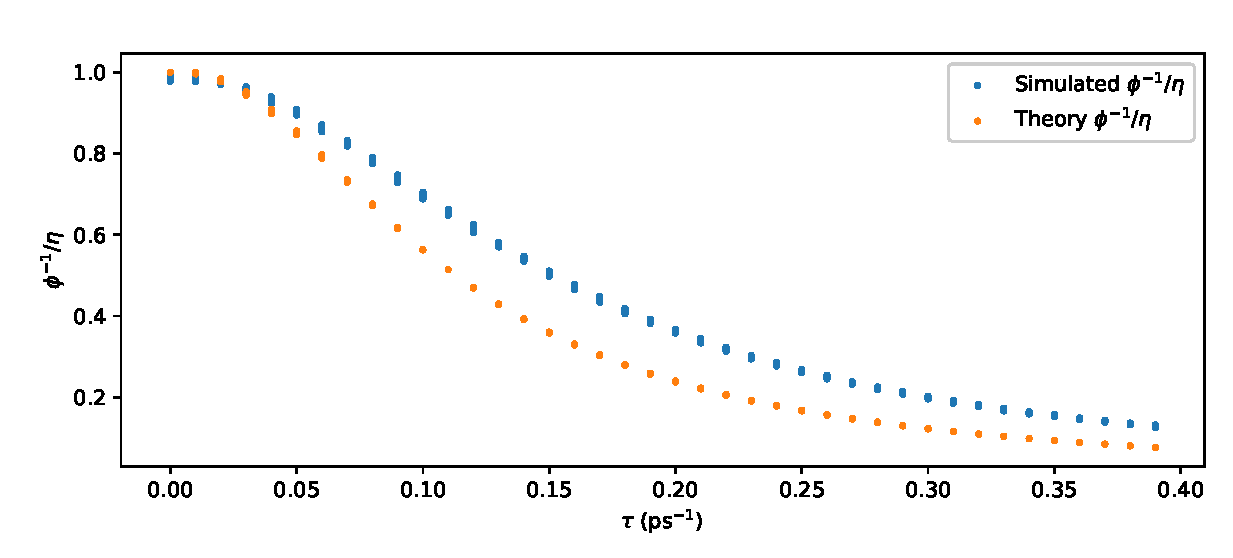
\includegraphics[width=1.0\textwidth]{theoretical_tau_ttf}
	\caption{}
	\label{fig:theoretical_tau_ttf}
\end{figure}

\section{something else}

The Markovian Langevin equation implicitly assumes that the correlation time of the Langevin noise term is infinitesimally small, that is to say, $\left< f(t_1) f(t_2) \right> = \sigma^2 \delta (t_1 - t_2)$. In Fourier space, this condition is equivelant to the statement that the power spectrum of the noise is uniform, $\left< \tilde{f}(\omega_1) \tilde{f}(\omega_2) \right> = 2 \pi \sigma^2 \delta(\omega_1 + \omega_2)$. However all real systems are bandlimited and in the case of surface dynamics the noise cutoff manifests as the phonon cutoff frequency of the substrate. Even in an idealised Langevin simulation, the spectrum of the simulated noise cannot excede $\frac{1}{2\delta{t}}$, where $\delta{t}$ is the timestep of the simulation, and so the effects of ommitting high frequency noise components need to be understood to be safely neglected. 

If no background potential is present, the solution to the Langevin equation may be expressed as a simple integral over a Green's function, $F(t)$, satisfying $\ddot{F} + \eta \dot{F} = \delta(t)$,

$$
x(t) = \frac{1}{m} \int_{-\infty}^t \diff{t'} f(t') F(t-t') \longrightarrow \tilde{x}(\omega) = \frac{1}{m} \tilde{f} \tilde{F}.
$$ 

In this case the removal of high frequency noise components in $\tilde{f}$ simply amounts to the removal of these same noise components from the trajectory of the particle. From this analysis it may be expected that high frequency noise components only affect the short time-scale motion of the particle but leave the macroscopic trajectory unchanged, as demonstrated in Figure \ref{fig:noise_trajectories}. However in the presence of an anharmonic background potential, the Langevin equation ceases to be linear in $x$ and the compounding of small differences between trajectories causes macroscopic divergence between trajectories which otherwise only differ in high frequency noise components. While this does not immediately imply that statistical properties taken over an ensemble of trajectories will be affected, one cannot assume that long-time scale observables are unaffected by high frequency noise in the non-linear case.

\begin{figure}
	\centering
	\includegraphics[width=0.8\textwidth]{noise_trajectories}
	\caption{A demonstration of how the introduction of bandlimited noise affects the trajectory of a particle.}
	\label{fig:noise_trajectories}
\end{figure}

\subsection{Evaluation of the effect of high frequency noise on the hopping rate of Sodium on Copper(001)} \label{sec:hopping_simulations}

A Langevin simulation was constructed using a potential energy surface extracted from a molecular dynamics model of Sodium adsorbed on Copper(001) as presented in \cite{Gil}. An exponential memory kernel of the form $K(t) = \frac{1}{\tau}\exp(-t/\tau)$ was introduced to control the bandwidth of the noise. The noise correlation time $\tau$ is related to the bandwidth of the noise through the relation $\tau = \frac{1}{2 \pi f_c}$ where $f_c$ is the frequency at which the power spectrum of the noise is reduced to half its peak value. 

A GLE simulation was run for $2\us$ for each value of $\eta\in\left[0.4, 0.8\right)\ips$ and $\tau\in\left[0, 0.4\right)\ps$ in steps of $0.01$ at a temperature of $300\K$. The simulated trajectories were used to calculate the long-time decay rate of the ISF as well as the decay rate of the total energy auto-correlation function. The results of these simulations are summarized in Figure \ref{fig:ttf_gamma}.

Figure \ref{fig:gamma_and_ttf_contours} demonstrates the non-trivial dependence of the system's time to forget and ISF decay rate on $\eta$ and $\tau$. From these results it is evident that correlations in the system's noise can have a strong effect on the hopping rate of the adsorbate. Although the ISF decay rate is a function of both $\eta$ and $\tau$, the alignment of the contours of $\phi^{-1}$ and $\Gamma$ shows that, for a given temperature and background potential, $\Gamma$ is parametrized by only one parameter, the systems time to forget, and is independent of the orthogonal parameter.

The relationship between $\Gamma$ and $\phi$ is shown in Figure $\ref{fig:gamma_and_ttf_scatter}$ and is observed to be linear in $\phi^{-1}$ apart from the $\phi^{-1} \rightarrow 0$ limit. This departure from linearity may be attributed to the probability of hopping being affected by the time to forget in this limit.  

\begin{figure}
	\centering
	\begin{subfigure}{1.0\textwidth}
		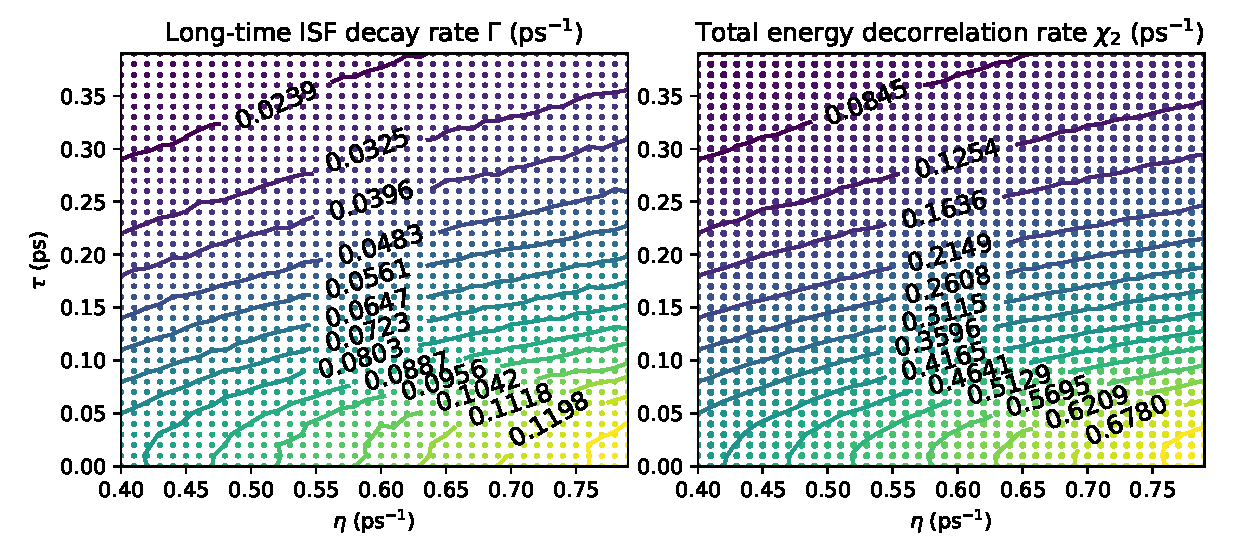
\includegraphics[width=1.0\textwidth]{gamma_and_ttf_contours}
		\caption{Contour plots of the long-time ISF decay rate, $\Gamma$, and the decay rate of the total energy auto-correlation function, $\chi_2$ as functions of $\eta$ and $\tau$. The alignment of the contours implies that, in this parameter regime, the pre-exponential factor of the hopping rate is solely a function of the system's `time to forget'.}
		\label{fig:gamma_and_ttf_contours}
	\end{subfigure}
	\begin{subfigure}{1.0\textwidth}
		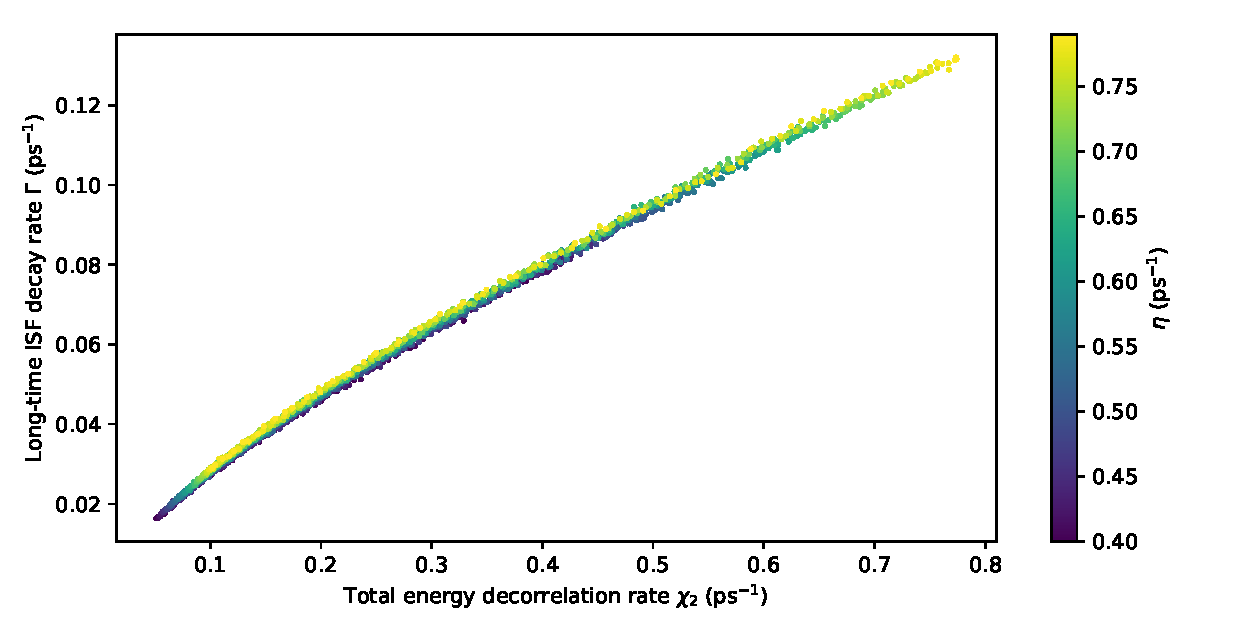
\includegraphics[width=1.0\textwidth]{gamma_and_ttf_scatter}
		\caption{The relationship between the kinetic energy decay rate and the ISF decay rate is observed to be linear except in the small $\chi_2$ limit. The colour of each marker is set by the value of $\eta$ for the simulation and further demonstrates that $\Gamma$ is not solely function of $\eta$.}
		\label{fig:gamma_and_ttf_scatter}
	\end{subfigure}
	\caption{}
	\label{fig:ttf_gamma}
\end{figure}

\subsection{Theoretical models of a system's time to forget} 

The time to forget of a system can be better understood through the study of some simple theoretical models. The simplest case of a particle with Langevin statistics in a flat potential has a time to forget of $\phi=\frac{1}{2\eta}$ whereas the introduction of a harmonic background potential, $V(x)=\frac{1}{2}m\omega_0^2x^2$, results in a longer time to forget of $\phi=\eta^{-1}$. This difference can be traced back to the fact that the energy of the particle in a harmonic well spends half its time in potential form where it remains unaffected by friction. If a noise cutoff is introduced to the harmonic system in the form of the aforementioned exponential memory kernel, things complicate considerably and the time to forget becomes a non-trivial function of $\eta$, $\tau$ and $\omega_0$. The functional form of these relationships depend on the exact pole structure of the Green's function of the system and its qualitive behaviour can vary drastically in a similar fashion to an under vs overdamped oscillator.

As a model for the corrugated periodic potential of a substrate, Figure \ref{fig:compare_theoretical_ttf} compares the time to forget of the corrugated potential to the time to forget of an equivalent harmonic well with the same curvature as the potential minimum of the corrugated potential of Section \ref{sec:hopping_simulations}. The results indicate that the time to forget of the harmonic well is only a reasonable approximation for low levels of $\tau$ with the error rapidly reaching 40\%. This is attributed to deviations of the corrugated potential from the harmonic potential becoming pronounced around the typical thermal energies at $300\K$. To be run again at lower temperatures. 

\begin{figure}
	\centering
	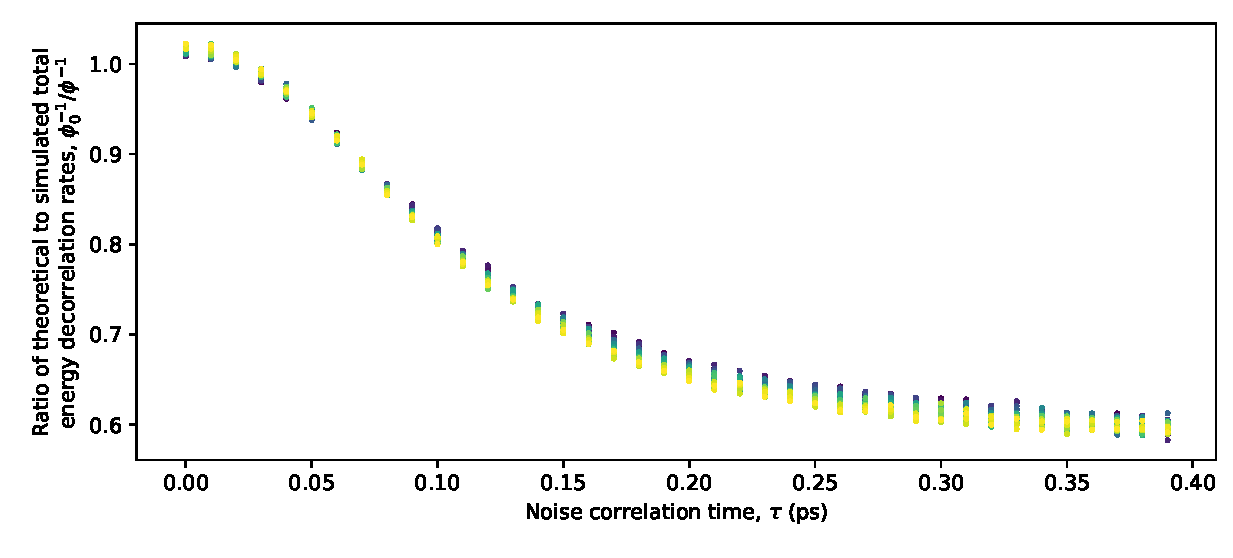
\includegraphics[width=1.0\textwidth]{theoretical_ttf_comparison}
	\caption{}
	\label{fig:compare_theoretical_ttf}
\end{figure}

\section{Temperature dependent friction and the effect of low frequency phonons}

While the upper bound of the phonon noise spectrum is set by the inter-atomic spacing of the lattice, the lower bound is set by the size of the substrate. The length of the substrate fixes a maximum phonon wavelength with a corresponding minimum vibrational frequency. While physical substrates are well approximated by an unbounded system, 3D molecular dynamics simulations are severly limited in system size due to computational cost. The paper by \ref{Gil} explores the ability of a Langevin simulation to fit a full 3D model of Na on Cu(001). This paper found that the friction parameter required to fit the observed data increased as a function of temperature. The 3D simulations in the aforementioned paper were performed with a crystal of size $8\times8\times8$ which suggests that these effects may be an artefect of finite system size. To test this hypothesis, the simulation setup was recreated across three separate system sizes, $8^3$, $16^3$ and $32^3$. Each system was randomly initialized and allowed to run for $10\ns$ for $200$ iterations with a cumulative runtime of $2\us$. It is important to re-initialize the substrate accross iterations so substrate energy can be shuffled between stable phonon modes. From each simulation, the ISF dephasing rate as a function of momentum transfer was calculated in the same fashion as described  

\begin{figure}
	\begin{subfigure}{1.0\textwidth}
		\centering
		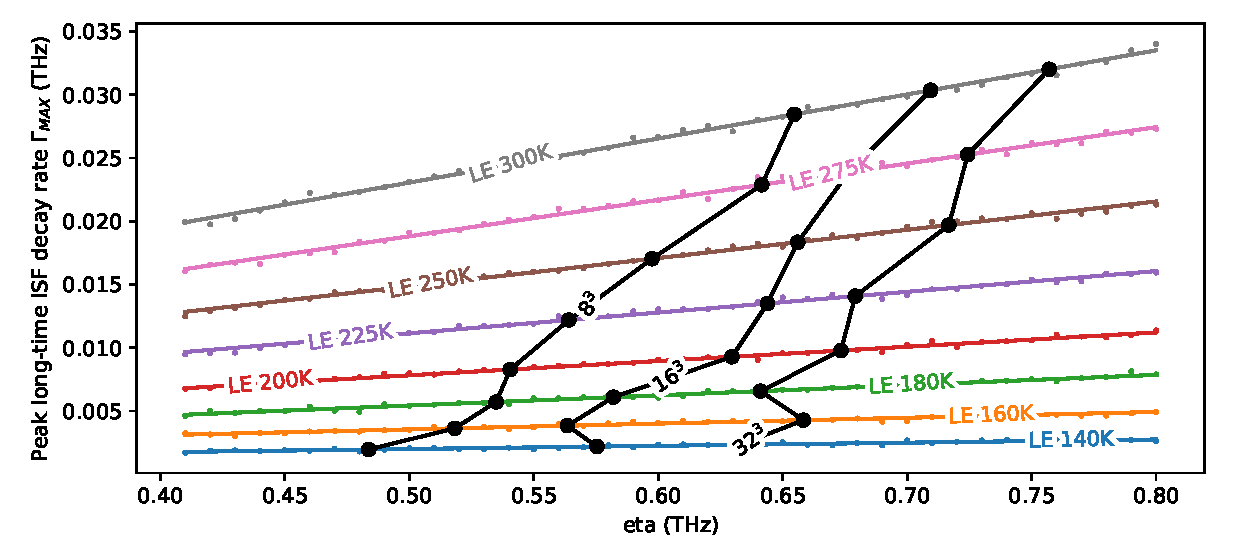
\includegraphics[width=1.0\textwidth]{md_vs_gle_gamma}
		\caption{}
		\label{fig:md_vs_gle_gamma}
	\end{subfigure}
	
	\begin{subfigure}{1.0\textwidth}
		\centering
		\includegraphics[width=1.0\textwidth]{md_temp_vs_eta}
		\caption{}
		\label{fig:md_temp_vs_eta}
	\end{subfigure}
\end{figure}

The potential energy surface isn't changed

\section{Summary}

$w_0=48$

test

\end{document}
